%use mybib.bib for bibliography. bibtex is used for bibliography
\documentclass[journal]{IEEEtran}
\usepackage[utf8]{inputenc}
\usepackage{graphicx}
\usepackage{cite}
\usepackage{longtable}
\usepackage{amsmath}
\usepackage{multirow}
\usepackage{multicol}
\usepackage{wrapfig}
\usepackage{float}
\usepackage{algorithmicx}
\usepackage{algpseudocode}
%\usepackage[section]{placeins}
%\usepackage{subcaption}
\usepackage{array}
\usepackage[export]{adjustbox}
\usepackage{tabu}
\usepackage{tabularx}
\usepackage{listings}
\usepackage{siunitx}
\usepackage{siunitx}
\usepackage{ wasysym }
\usepackage[usenames, dvipsnames]{color}
\usepackage{diagbox}


%%%%%%%%%%%%%%%%%%%%%%%%%%%%%%%%%%%%%%%%%%%%%%%%%%%%%


\ifCLASSINFOpdf

\else

\fi


\hyphenation{op-tical net-works semi-conduc-tor}


\begin{document}

\title{A Graph Search Based Energy Management Strategy for Grid-Connected Distributed Energy Resources Considering Present and Future System Status}

\author{\IEEEauthorblockN{Alvi Newaz\IEEEauthorrefmark{1}, Md. Omar Faruque\IEEEauthorrefmark{0}}
\IEEEauthorblockA{\\The Department of Electrical and Computer Engineering at the FAMU-FSU College of Engineering \\ Center for Advanced Power Systems, Florida State University \\
2000 Levy Avenue, Tallahassee, FL., USA.
%Wherever\\
Email: an15m@my.fsu.edu\IEEEauthorrefmark{1}}}


\maketitle
\IEEEpeerreviewmaketitle

\begin{abstract}
This paper presents a real-time  energy management system (EMS) for distribution systems or microgrids containing distributed energy resources (DERs). The EMS aims to optimize the use of dispatchable grid-connected DERs to achieve the minimum cost of operation while taking into consideration line constraints and present and future status of the grid. To achieve this the ESM algorithm generates a graph based on the present and forecasted data and uses the A* search algorithm to find the minimum cost. The algorithm is validated using off-line phasor simulation using pricing schemes from New York Independent System Operator (NYISO) and Pacific Gas and Electric (PG\&E) and system data from the sunshine state solar grid initiative (SUNGRIN) report. The real-time controller hardware in the loop (CHIL) validation of the algorithm is performed by simulating a full electromagnetic transient model of the system in a digital real-time simulator. The results are comparable to the offline simulation and show significant cost savings due to considering future status of the grid compared to optimizing based on only the current system status.

\end{abstract}

\section{Introduction} \label{sec:intro}
With the increase in penetration of Distributed Energy Sources (DERs) in the electric distribution network level, it is becoming increasingly difficult to establish stable network operation based on the traditional centralized control scheme of the grid \cite{WHY}. Especially the integration of photovoltaic and wind generation in the low voltage and medium voltage is making the grid less predictable and difficult to control. In general, today's power grid operation is based on day-ahead planning, in which the balancing of demand and generation of the grid is planned to determine optimum set points of operation. In case of a mismatch with the day ahead planning and real scenario a real-time control is usually put in place to take corrective actions \cite{WHY2}. Due to the increasing uncertainty in the grid these approaches are resulting in the grid operating sub-optimally based on a day-ahead planned control strategy \cite{WHY2}. To tackle this uncertainty of DER integration, integrating energy storage into the grid has been proposed by several researchers \cite{WHY2,ESI1,ES2,ES3}. 
This paper proposes a graph search based control strategy to control multiple energy storage system (ESS). The goal of the control strategy is to provide the most cost optimum operation of the energy storages while providing peak shaving functionality. In \cite{IM1} the researchers propose a control strategy to smooth out the output of a wind farm using the help of ESS. The control makes sure that the output of the wind farm matches a previously predicted output profile. It optimizes the use of the ESS over a prediction horizon to get better results. In \cite{IM2} researchers optimize ESS connected to a distribution feeder hosting a significant amount of renewable energy resources. The objective of the research is to most cost optimally operate the ESS. Reference \cite{IM3} looks at the optimum use of ESS from a transmission grid standpoint. And the researchers in \cite{IM4} show an IEE 14 bus system based proof of concept of an optimum power flow solution considering ESS. From the discussion thus far it is evident that the integration of RES into the distribution grid is creating some new challenges for grid operation and there has been significant research done to show that ESS can be deployed as a possible solution to counteract the uncertainties introduced to the grid by RES integration. To most optimally control the ESS there needs to be a real-time algorithm which takes into account current and predicted system status \cite{gupta_francis_ospina_newaz_2018}. In case of multiple ESS connected to a distribution system, it is also imperative that the solution obtained does not violate any system constraints \cite{rt4}. So an optimum solution considering both system architecture and constraints and current and predicted system status is necessary to most cost optimally control the ESS.

\section{Problem Formulation} \label{sec:problem_formulation}
Fig. \ref{fig:controller-setup} shows a simplified top-level architecture of the control problem. Here, the controller is in charge of managing the energy of the energy storage and utility-owned generator of a distribution feeder. This is an example feeder comprised of five buses, two PVs (Pv1, PV2), four loads (D2, D3, D4 \& D5), four lines (L1, L2, L3 \& L4),  two energy storage (ES1, ES2), and one utility-owned generator (G). The energy management system  (EMS) shown in  Fig. \ref{fig:controller-setup} is taking the system status, forecasts, and RTP data as input and determining the power output of the controllable DERs, which in this case are the two energy storage and the utility-owned generator.

\begin{figure}
\centering
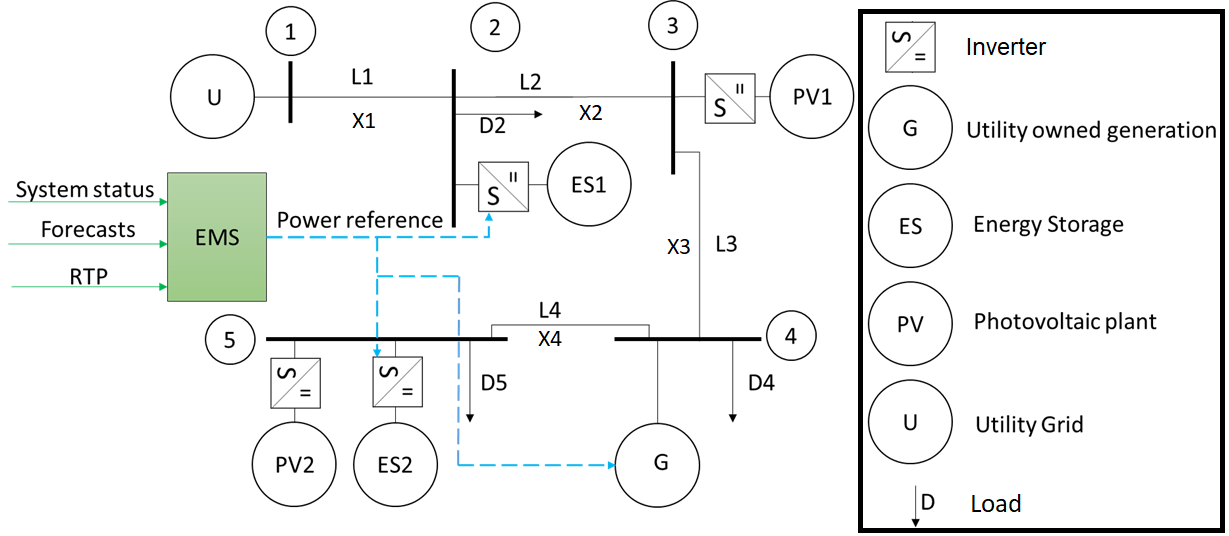
\includegraphics[width = \linewidth]{figs/A82/controller_setup2.png}
\caption{Simplified top-level controller architecture}
\label{fig:controller-setup}
\end{figure}

To incorporate the future forecasts and RTP as well as the current system status a graph is constructed from both the present and future status of the system. Fig. \ref{fig:F1_1_Dis} represents a simple example graph which is constructed assuming relevant forecasts and RTP is available for the system to generate states 15, 30 and 45 minutes in the future. . The values on top of the figure represent time. T = 0 represents the present and T = 15, 30 and 45 represents future states 15, 30 and 45 minutes in the future. The boxes with numbers inside are the nodes of the graph. The numbers represent the percentage of total energy storage (ES) capacity available to the system. The arrows represent the edges of the graph. In this case the edges are unidirectional. This is because it is impossible to return to a past node from a future node. The edges represents the cost of going from one node to the another. The graph is constructed considering an operation between 20\% to 80\% of total ES capacity and discretization steps of 20\%. It is also considered that the system has the capacity to discharge 40\% of the total energy capacity at most and charge up to 20\% of the total energy capacity at most within 15 minutes. Taking all these things into consideration the graph in fig. \ref{fig:F1_1_Dis} is generated and the problem that needs to be solved is to find the most cost optimum path to go from the starting node at T = 0 to any node at T = 45 while maintaining system constraints.

% The cost optimum solution is found by finding the optimum path in a graph search problem formulated to reflect different operation scenarios of the system. Fig. \ref{fig:F1_1_Dis} represents a simple example of the graph search formulation of the problem. The values on top of the figure represent the current time-step. The values inside the boxes represent the percentage of total energy storage (ES) capacity available in the system. These boxes are the nodes of the graph. The arrows from one box to the next represent the edges of the graph. It is assumed that the system power demand is constant between time steps. The system status at T=0 is known from the current measurement. The nodes at T=15, T=30, and T=45 are created based on forecasted values. The target of the solution is to find the most cost-optimum path to reach T=45 based on the predictions available. 

\begin{figure}[!h]
\centering
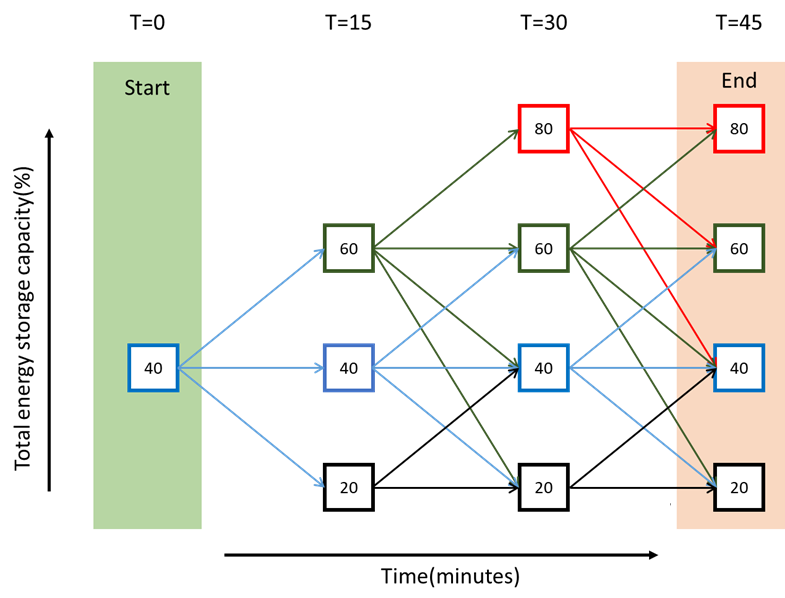
\includegraphics[width = .8\linewidth]{figs/A82/A8_graph_22.png}
\caption{Graph formulation}
\label{fig:F1_1_Dis}
\end{figure}

\section{Energy Management Solution Combining Graph Search and Quadratic Programming}
To solve the problem mentioned in Section \ref{sec:problem_formulation} a combination of two optimization processes are happening. The first process in in charge of finding the most cost optimum solution to go from one node of the graph to another. This process formulates the cost function of the edges of the graph as a cost minimization problem which is solved using quadratic programming. The second process is in charge of finding the most cost optimum path through the graph generated using the optimized edges from the first process. This process uses the A* search algorithm for this task. The quadratic programming formulation of edge costs and the A* algorithm is described in detail in this chapter.

% The cost function of the edges of the graph is formulated as a minimization problem which is solved using quadratic programming. To find the optimum path through the graph the A* path finding  algorithm is used. In this case   This is done u

% The graph search, in this case, is also done using the A* search algorithm described in chapter \ref{A8_cahp}, Algorithm 1. The difference, in this case, is that for calculating the cost of each edge of the graph a quadratic programming problem is solved. So unlike the single energy storage scenario here, two optimization processes are happening. First, the optimum solution to go from the parent graph nodes to the child graph nodes are optimized using quadratic programming. Then, the optimized graph edges are used to find an optimum solution based on forecasts and current states of the system while considering system constraints. 

\subsection{DC Power-Flow}
The regular AC power-flow is non-linear. Using the non-linear equations of AC power-flow to derive the system constraints would make the problem of calculating the edge cost of the graphs a non-linear problem. To linearize the problem DC power flow \cite{DC_PF1} is used instead. This results in a linear minimization problem for cost calculation that can be solved quickly. In DC power-flow the losses due to resistive elements in the power line are ignored. Also, some approximation are made on the fact that the voltage magnitude and angle difference between adjacent nodes are very small and the node voltages are usually near 1 p.u.. A small example is presented using the two bus system shown in Fig. \ref{fig:DC_PF}. The voltage magnitude \& angle of of Bus1 and Bus2 are $v_1$ \& $\delta_1$ and $v_2$ \& $\delta_2$ respectively. Bus1 supplies power $P_1$ and Bus2 consumes power $P_2$. The kine admittance is defined as $y$ with susceptance $b$ and conductance $g$. Using these parameters the AC powerflow of the two bus system can be expressed using (\ref{eq:AC_PF_1}) and (\ref{eq:AC_PF_2}).
% DC power flow  
% DC power flow is a linearized 
% Part of the constraints used in the edge cost function is derived from DC power flow \cite{DC_PF1}. DC power flow is a linearized approximation of the regular AC power flow which ignores losses due to resistive elements of the power line. It also considers some approximations based on the fact that the voltage angle difference between two adjacent nodes are usually minuscule and their magnitudes are usually near the value of 1 P.U. . For example let us consider the two bus systems shown in Fig. \ref{fig:DC_PF}. Bus1 has a per unit voltage magnitude of $v_1$ and angle of $\delta_1$. Bus2 has a per unit voltage magnitude of $v_2$ and angle of $\delta_2$. The power supplied by Bus1 is $P_1$ and the power received by Bus2 is $P_2$. $y$ is the admittance of the line with conductance $g$ and susceptance $b$. In traditional AC power-flow $P_1$ and $P_2$ can be defined as:
\begin{equation}
\label{eq:AC_PF_1}
    P_1 = +gv_1( v_1 - v_2 cos(\delta_1 - \delta_2)) - v_1v_2bsin(\delta_1 - \delta_2)
\end{equation}
\begin{equation}
\label{eq:AC_PF_2}
    P_2 = -gv_2( v_2 - v_1 cos(\delta_1 - \delta_2)) - v_1v_2bsin(\delta_1 - \delta_2)
\end{equation}

If we neglect loss due to resistive elements (\ref{eq:AC_PF_1}) and (\ref{eq:AC_PF_2}) can be reduced to (\ref{eq:DC_PF_1}) \cite{DC_PF1}.

\begin{equation}
\label{eq:DC_PF_1}
P_1 \approx P_2 \approx - v_1v_2bsin(\delta_1 - \delta_2)
\end{equation}

Considering $v_1 \approx v_2 \approx 1$ and $\delta_1 \approx \delta_2$ equation (\ref{eq:DC_PF_1}) can be further reduced to
\begin{equation}
\label{eq:DC_PF_2}
P_1 \approx P_2 \approx -b(\delta_1 - \delta_2)
\end{equation}

Finally using the relation $-b \approx 1/x$ we get (\ref{eq:DC_PF_3}) from   (\ref{eq:DC_PF_2}).

\begin{equation}
\label{eq:DC_PF_3}
P_1 \approx P_2 \approx (\delta_1 - \delta_2)/x
\end{equation}

Here, $x$ is the reactance of the line between BUS1 and BUS2. Equation (\ref{eq:DC_PF_3}) represents the DC power-flow approximation of (\ref{eq:AC_PF_1}) and (\ref{eq:AC_PF_2}) \cite{DC_PF1}.

\begin{figure}[!ht]
\centering

\includegraphics[width = 0.6\linewidth]{figs/A82/DC_PF.png}
\caption{Simple two bus system}
\label{fig:DC_PF}
\end{figure}

\subsection{Edge Cost Formulation}
The DC power-flow approximation in (\ref{eq:DC_PF_3}) is used to formulate the edge cost of the graph as a minimization problem which has a quadratic cost function and linear constraints. The cost function is shown in (\ref{eq:A2_CF}).
% The approximation used in (\ref{eq:DC_PF_3}) converts the non-linear AC power-flow equations into a linear equation. This facilitates formulating the equations to calculate the edge cost of the graph search problem as a quadratic program possible. Equation (\ref{eq:A2_CF}) shows the cost function.
\begin{multline}
\label{eq:A2_CF}
C_{total} = (P_{grid} * RTP + \sum_{n=1}^{N_{es}} (|P_{es}(n)|*r_{es}(n)) \\+
\sum_{m=1}^{N_{gen}}(A(m)*P_{gen}(m)^2 + B(m)*P_{gen}(m)))*\Delta T
\end{multline}
Here, $C_{total}$, $P_{grid}$ and $RTP$ represents the total cost of an edge, power drawn from the grid and the real-time price respectively.

 $N_{es}$ is the total number of energy storage in the system. $|P_{es}(n)$ is the power supplied by the $n^{th}$ energy storage. $r_{es}(n)$ is the levelized cost of using energy for the $n^{th}$ energy storage. $r_{es}(n)$ is calculated using (\ref{eq:R_ESS}). $N_{gen}$ is the total number of traditional generators in the system. $P_{gen}(m)$ is the power supplied by the $m^{th}$ generator. $A(m)$ and $B(m)$ are the constants used to calculate the operating cost of the $m^{th}$ generator \cite{saadat1999power}. The constant cost of operating a generator is ignored in this case as it is a constant cost and can not be reduced through optimization. $\Delta T$ signifies time in seconds between the parent and child node. The constraints of the cost function are defined by equations (\ref{eq:A2_EQ2}), and (\ref{eq:A2_EQ3}).
% \begin{equation}
% \label{eq:A2_EQ1}
% \sum_{n=1}^{N_{es}}P_{es}(n) + P_{grid} + \sum_{m=1}^{N_{gen}}P_{gen}(m) = \sum_{k=1}^{N_{load}}P_{load}(k) - \sum_{l=1}^{N_{PV}}P_{PV}(l)
% \end{equation}
% Here, $N_{load}$ is the total number of loads in the system. $P_{load}(k)$ is the power supplied by the $k^{th}$. $N_{PV}$ is the total number of PVs in the system, and 
\begin{equation}
\label{eq:A2_EQ2}
\sum_{n=1}^{N_{es}}P_{es}(n) = \Delta ES / \Delta T
\end{equation}
Equation (\ref{eq:A2_EQ2}) represents the equality constraints imposed by the graph search. As seen in Fig. \ref{fig:F1_1_Dis}, going from a parent node to a child node signifies a percentage change in the total energy storage capacity of the system. Here, $\Delta ES$ signifies the total change in energy required to match the percentage change in the total energy storage capacity determined by the graph edge. $\Delta ES$ is divided by $\Delta T$ to convert from energy to power. These constraints ensure that the power supplied or absorbed by the energy storage match the graph edge.
\begin{equation}
\label{eq:A2_EQ3}
P = P_{load} - P_{PV} - P_{es} = h*\Delta \delta 
\end{equation}
Equation (\ref{eq:A2_EQ3}) represents the equality constraints generated from DC power-flow. It is a matrix representation of (\ref{eq:DC_PF_3}) \cite{DC_PF1}. Here, $h$ is the admittance matrix of the system. $\Delta \delta$ is the matrix of angle difference between adjacent busses. The components of bus power vector P are:\\
$P_{load} =$ Power requirements of load.\\
$P_{PV} =$ Power supplied by PV.\\
$P_{es} =$ power supplied by es.\\


The inequality constants are expressed using equations (\ref{eq:A2_IEQ1}), (\ref{eq:A2_IEQ2}) and (\ref{eq:A2_IEQ3}).
\begin{equation}
\label{eq:A2_IEQ1}
0 \leq P_{gen}(m) \leq \overline{P_{gen}(m)}, \quad m = 1, 2, 3, ... , N_{gen}
\end{equation}
Equation (\ref{eq:A2_IEQ1}) represents the inequality constraints rising from the power limits of the traditional generators. $P_{gen}(m)$ is the power generated by the $m^{th}$ generator, and $\overline{P_{gen}(m)}$ is the upper limit of generation for the $m^{th}$ generator. $N_{gen}$ is the total number of generators available. This constraint ensures that all available generators in the system generates power within the operating limit of the respective generator.
\begin{multline}
\label{eq:A2_IEQ2}
\underline{ES(n)} \leq ES_{current}(n)+(P_{es}(n)*\Delta T) \leq \overline{ES(n)}, \\ n = 1, 2, 3, ... , N_{es}
\end{multline}
Equation (\ref{eq:A2_IEQ2}) represents the inequality constraints pertaining to the upper and lower state of energy bounds of energy storage. $\underline{ES(n)}$ is the lower bound of stored energy, and $\overline{ES(n)}$ is the upper bound of stored energy for the $n^{th}$ energy storage. $ES_{current}(n)$ is the energy stored in the energy storage at the parent node. $P_{es}(n)$ is the power supplied by the $n^{th}$ energy storage. A negative value for $P_{es}(n)$ signifies charging and a positive value signifies discharging. $P_{es}(n)$is multiplied by $\Delta T$ to convert it from power to energy.
\begin{equation}
\label{eq:A2_IEQ3}
\underline{P_{ES}(n)} \leq P_{es}(n) \leq \overline{P_{ES}(n)}, \quad n = 1, 2, 3, ... , N_{es}
\end{equation}
Equation (\ref{eq:A2_IEQ3}) shows the inequality constraints pertaining to the charging and discharging power rating of the energy storage. $\underline{P_{ES}(n)}$ is the highest charging power rating  and $\overline{P_{ES}(n)}$ is the highest discharging power rating of the $n^{th}$ energy storage. Equations (\ref{eq:A2_IEQ2}) and (\ref{eq:A2_IEQ3}) makes sure that all the energy storage in the system operate within their limits.

Combining all the equations from (\ref{eq:A2_CF}) to (\ref{eq:A2_IEQ3}) the full form of the quadratic programming formulation to solve the edge cost is as follows:\\
Minimize:
\begin{multline}
\label{eq:multi_all_in1}
(P_{grid} * RTP + \sum_{n=1}^{N_{es}} (|P_{es}(n)|*r_{es}(n)) + \\ \sum_{m=1}^{N_{gen}}(A(m)*P_{gen}(m)^2 + B(m)*P_{gen}(m)))*\Delta T
\end{multline}
Subject to:\\

$\sum_{n=1}^{N_{es}}P_{es}(n) = \Delta ES / \Delta T$

$P = P_{load} - P_{PV} - P_{es} = h*\Delta \delta $

$0 \leq P_{gen}(m) \leq \overline{P_{gen}(m)}$

$\underline{ES(n)} \leq ES_{current}(n)+(P_{es}(n)*\Delta T) \leq \overline{ES(n)}$

$\underline{P_{ES}(n)} \leq P_{es}(n) \leq \overline{P_{ES}(n)}$\\

Where,

$m = 1, 2, 3, ... , N_{gen}$, and $n = 1, 2, 3, ... , N_{es}$.\\

When calculating the $G_{cost}[child]$ of Algorithm 1, this minimization problem is solved to get the cost of the edges of the graph.
\subsection{Heuristic Cost Calculation}
The heuristic cost calculation function calculates the heuristic used by the A* search algorithm. In this case the heuristic cost is calculated using (\ref{eq:multi_hu1}).
\begin{equation}
\label{eq:multi_hu1}
    C_H(t) = \sum_{n=t}^{end} C_{best}(n)
\end{equation}

Here, $C_H(t)$ is the heuristic cost for time $t$ and $C_{best}(n)$ is the best possible cost at time $n$. The best possible cost is calculated by relaxing some of the constraints for (\ref{eq:multi_all_in1}). The cost function is kept the same. The constraints pertaining to energy storage availability from (\ref{eq:A2_IEQ2}) is removed. The constraint defined by (\ref{eq:A2_EQ2}) are also removed. The minimization problem solved to find $C_{best}(n)$ fot the time $n$ is as follows:\\
Minimize:
\begin{multline}
\label{eq:multi_hu2}
C_{best}(n)=(P_{grid} * RTP + \sum_{n=1}^{N_{es}} (|P_{es}(n)|*r_{es}(n)) +\\ \sum_{m=1}^{N_{gen}}(A(m)*P_{gen}(m)^2 + B(m)*P_{gen}(m)))*\Delta T
\end{multline}
Subject to:\\

$\sum_{n=1}^{N_{es}}P_{es}(n) = \Delta ES / \Delta T$


$0 \leq P_{gen}(m) \leq \overline{P_{gen}(m)}$


$\underline{P_{ES}(n)} \leq P_{es}(n) \leq \overline{P_{ES}(n)}$\\

Where,

$m = 1, 2, 3, ... , N_{gen}$, and $n = 1, 2, 3, ... , N_{es}$

\subsection{Using A* to Search the Graph}

\textbf{Algorithm 1:} A* search algorithm

\begin{algorithmic}[1]
\label{al:1}
% \Function{heuristic\_estimate}{$a,b$}
%     \State $hCost := \sum_{n=a}^b D(n)*R_{best}(n) $
%     \State \Return $hCost$
% \EndFunction

% \Function{gCost\_calc}{$p,c$}
%     \State $C_{actual}(pc) := C_{ESS}(pc)+C_{GRID}(t)+C_{best}(p)$
%     \State \Return $C_{actual}(pc)$
% \EndFunction

\Function{A*}{$start, goal$}
\State $Closed\_Set = \{\}$ \Comment{Set of evaluated nodes}
\State $Open\_Set = \{Start\}$ \Comment{Set of already discovered nodes which have not been evaluated. Initially,  the start node is discovered.}
\State $F\_cost[Start] = \infty$
\While{$Open\_Set$ is not empty}
    \State $Current\_Node = $ node in $Open\_Set$ with lowest $F\_cost$
    \If{$Current\_Node$ == goal}
      \State  \textbf{break} 
    \EndIf
    \For {Each child node of $Current\_Node$}
        \If{Child node in $Closed\_Set$}
            \State \textbf{continue}
        \EndIf
        \If{Child node in $Open\_Set$}
            \If{$G\_cost[child]$ $\geq$ $G\_cost$ already in $Open\_Set$}
                \State \textbf{continue}
            \EndIf
        \EndIf
        \State $Best\_Parent[child] = Current\_Node$
        \State $F\_cost[child] = G\_cost[child] + H\_cost[child]$
        \State $Open\_Set.add(child)$ \Comment{Add child node to $Open\_Set$}

    \EndFor
    \State $Closed\_Set.add(Current\_Node)$ \Comment{Add $Current\_Node$ to $Closed\_Set$}
    \State $Open\_Set.remove(Current\_Node)$ \Comment{Remove $Current\_Node$ From $Open\_Set$}
\EndWhile
\State $Best\_Path = \{ \}$ \Comment{$Best\_Path$ is the most efficient path to get to the goal node.}
\While{$Best\_Parent[Current\_Node] != Start$}
    \State $Current\_Node = Best\_Parent[Current\_Node]$
    \State $Best\_Path.add(Current\_Node)$ \Comment{Add $Current\_Node$ to $Best\_Path$}
\EndWhile
\State \Return $Best\_Path$
\EndFunction
\end{algorithmic}

\section{Test System for Cost Optimization}
To test the proposed algorithm a modified version of the feeder used in chapter \ref{A8_cahp} was used. Fig. \ref{fig:modified_feeder_2} shows the modified feeder. The only differences here are a generator is added to bus B20050P, and the energy storage added to bus B20080P to represent a microgrid at that location. The generator has a rated maximum capacity of 2000 kW. The energy storage properties are shown in Table \ref{tab:es}. Detailed descriptions about the other components of the feeder can be found in Chapter \ref{A8_cahp}, section \ref{sys}, and in Chapter \ref{CVC}, section \ref{sec:cvc_test_system}.
\begin{figure}[!ht]
\centering
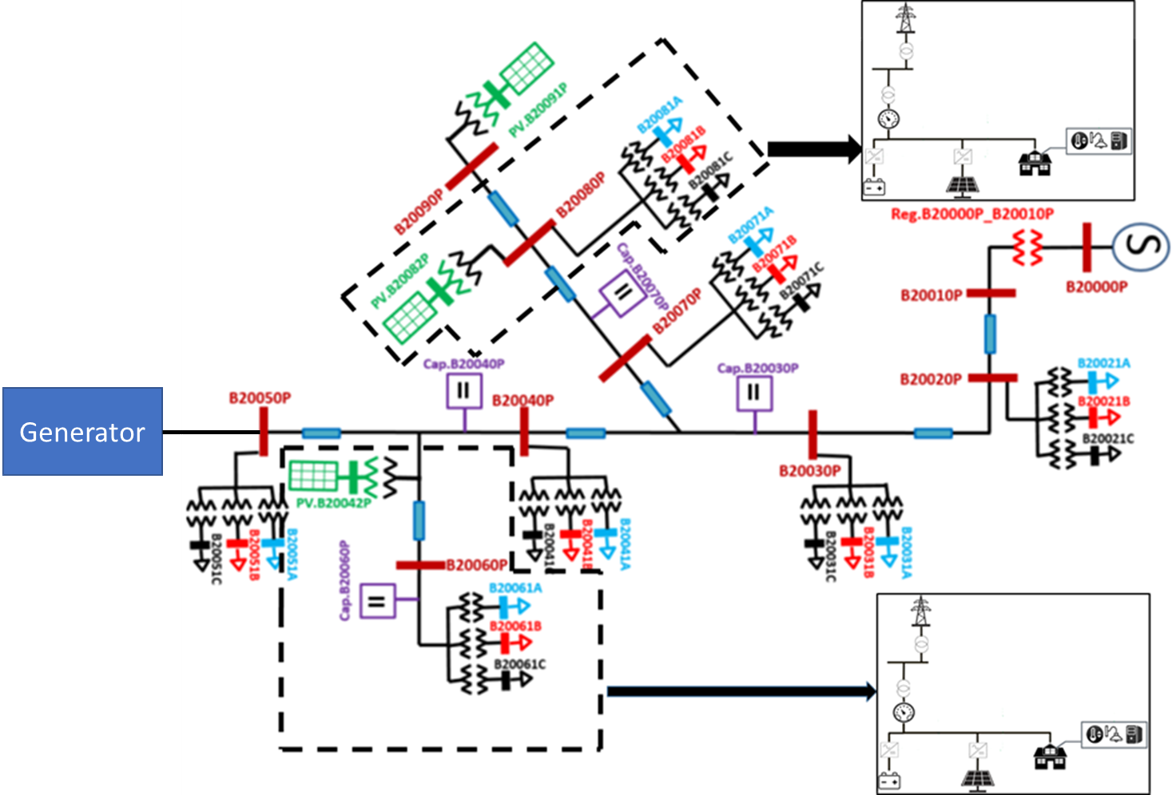
\includegraphics[width = \linewidth]{figs/A82/modified_feeder_2.png}
\caption{Distribution system used in simulation}
\label{fig:modified_feeder_2}
\end{figure}

\begin{figure}[!ht]
\centering
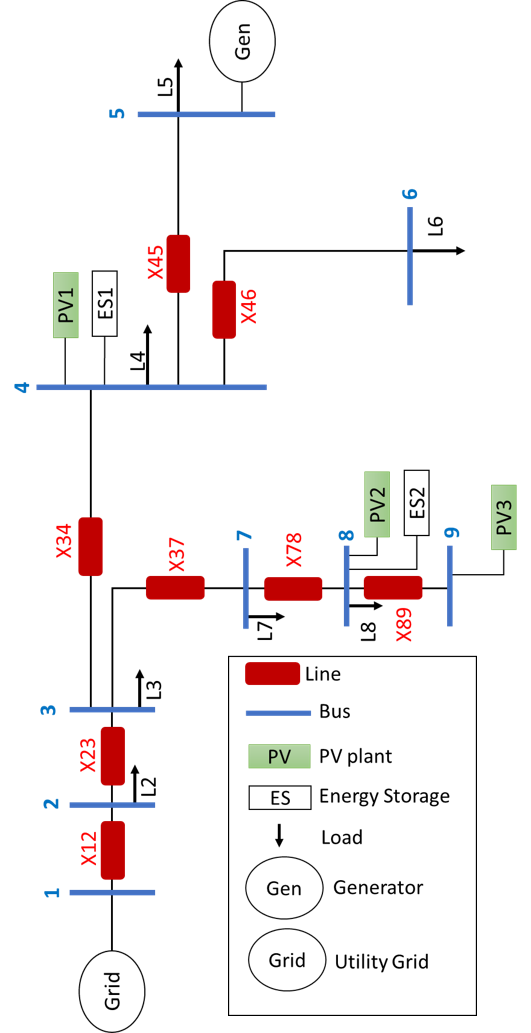
\includegraphics[width = .5\linewidth, angle = 270]{figs/A82/Grid_setup.png}
\caption{Simplified one-line diagram of the distribution system used in simulation.}
\label{fig:one_line}
\end{figure}

Fig. \ref{fig:one_line} represents a simplified one-line diagram of the feeder. Here buses 1, 2, 3, 4, 5, 6, 7, 8, and 9 represents buses B20010P, B20020P, B20030P, B20040P, B20050P, B20060P, B20070P, B20080P, and B20090P from Fig. \ref{fig:modified_feeder_2}. X12, X23, X34, X45, X46, X37, X78 and X89 are the reactance of the lines between buses 1 \& 2, 2 \& 3, 3 \& 4, 4 \& 5, 4 \& 6, 3 \& 7, 7 \& 8, and 8 \& 9 respectively. L2, L3, L4, L5, L6, L7, and L8 are the loads connected to the buses 2, 3, 4, 5, 6, 7, and 8. Pv1 \& ES1, PV2 \& ES2 are the PV \& ES connected to bus 4 and bus 8. PV3 is the PV connected to bus 9. The quadratic problem formulation for determining the edge cost according to (\ref{eq:multi_all_in1}) is as follows:\\
minimize:
\begin{multline}
\label{eq:multi_all_in1_sys}
    ( P_{grid}*rtp + |(P_{es}(1)*r_{es}(1)| + |(P_{es}(2)*r_{es}(2)| \\ + A*P_{Gen}^2 + B*P_{Gen} )*\Delta T
\end{multline}
Subject to:\\

$P_{es}(1)+P_{es}(2) = \Delta ES / \Delta T$

$(\delta_1 - \delta_2)/X_{12} = P_{Grid}$

$(\delta_2 - \delta_1)/X_{12}+ (\delta_2 - \delta_3/X_{23} = P_{L2}$

$(\delta_3 - \delta_2)/X_{23}+(\delta_3 - \delta_4)/X_{34}+(\delta_3 - \delta_7)/X_{37} = P_{L3}$

$(\delta_4 - \delta_3)/X_{34}+(\delta_4 - \delta_4)/X_{45}+(\delta_4 - \delta_6)/X_{46}=P_{L4} -$

$P_{PV1} - P_{es}(1) - P_{PV}(1)$

$(\delta_5 - \delta_4)/X_{45} = P_{L5}-P_{Gen}$

$(\delta_6 - \delta_4)/X_{46} = P_{L6}$

$(\delta_7 - \delta_3)/X_{37} + (\delta_7 - \delta_8)/X_{78}  = P_{L7}$

$(\delta_8 - \delta_7)/X_{78} + (\delta_8 - \delta_9)/X_{89}  = P_{L8} - P_{es}(2) - P_{PV}(2)$

$(\delta_9 - \delta_8)/X_{89} = -P_{PV}(3)$

$0 \leq P_{Gen} \leq \overline{P_{Gen}}$

$\underline{ES(1)} \leq ES_{current}(1)+(P_{es}(1)*\Delta T) \leq \overline{ES(1)}$

$\underline{ES(2)} \leq ES_{current}(2)+(P_{es}(2)*\Delta T) \leq \overline{ES(2)}$

$\underline{P_{ES}(1)} \leq P_{es}(1) \leq \overline{P_{ES}(1)}$

$\underline{P_{ES}(2)} \leq P_{es}(2) \leq \overline{P_{ES}(2)}$\\

The heuristic cost is calculated using (\ref{eq:multi_hu1}). The formulation of (\ref{eq:multi_hu2}) is shown in (\ref{eq:multi_all_in1_sys_hu}).\\
minimize:
\begin{multline}
\label{eq:multi_all_in1_sys_hu}
    ( P_{grid}*rtp + |(P_{es}(1)*r_{es}(1)| + |(P_{es}(2)*r_{es}(2)| \\ + A*P_{Gen}^2 + B*P_{Gen} )*\Delta T
\end{multline}
Subject to:

$(\delta_1 - \delta_2)/X_{12} = P_{Grid}$

$(\delta_2 - \delta_1)/X_{12}+ (\delta_2 - \delta_3/X_{23} = P_{L2}$

$(\delta_3 - \delta_2)/X_{23}+(\delta_3 - \delta_4)/X_{34}+(\delta_3 - \delta_7)/X_{37} = P_{L3}$

$(\delta_4 - \delta_3)/X_{34}+(\delta_4 - \delta_4)/X_{45}+(\delta_4 - \delta_6)/X_{46}=P_{L4} -$

$P_{PV1} - P_{es}(1) - P_{PV}(1)$

$(\delta_5 - \delta_4)/X_{45} = P_{L5}-P_{Gen}$

$(\delta_6 - \delta_4)/X_{46} = P_{L6}$

$(\delta_7 - \delta_3)/X_{37} + (\delta_7 - \delta_8)/X_{78}  = P_{L7}$

$(\delta_8 - \delta_7)/X_{78} + (\delta_8 - \delta_9)/X_{89}  = P_{L8} - P_{es}(2) - P_{PV}(2)$

$(\delta_9 - \delta_8)/X_{89} = -P_{PV}(3)$

$0 \leq P_{Gen} \leq \overline{P_{Gen}}$

$\underline{P_{ES}(1)} \leq P_{es}(1) \leq \overline{P_{ES}(1)}$

$\underline{P_{ES}(2)} \leq P_{es}(2) \leq \overline{P_{ES}(2)}$\\


Both (\ref{eq:multi_all_in1_sys}), and (\ref{eq:multi_all_in1_sys_hu}) are solved using the embotech ECOS solver \cite{ecos}. 

\section{Offline Simulation and Results}
The process used for the offline simulation is the same as Chapter \ref{A8_cahp}. The feeder components use the same data as chapter \ref{A8_cahp} as well. Fig. \ref{fig:OFFLINE1_NM_ES} shows the offline simulation result for the energy storage using a NYISO based RTP. The $r_{es}(1)$ and $r_{es}(2)$ values are 5 cents/kWh and 7 cents/kWh. The other properties of the energy storage are the same as table \ref{tab:es}. The solid red line is ES1 SOC, the dashed blue line is ES2 SOC and the dotted black line is the RTP.
As it can be seen from fig. \ref{fig:OFFLINE1_NM_ES} they behave as expected. Both ES1 and ES2 charge during low price points and discharge during high price points. Fig. \ref{fig:GEN_COST_CURVE} shows the cost curve for the generator. The A and B values for the generator are 0.001\$ and 0.0001\$. Fig. \ref{fig:OFFLINE1_NM_Gen} shows the response of the energy provided by the generator and the grid. The solid red line is the energy supplied by the generator. The dashed blue line is the energy supplied by the grid and the dotted black line is RTP. It can be seen that during high price point the generator supplies energy. There is also a significant dip in the grid energy supply during the high price points. This signifies that the algorithm is behaving as expected.
Fig. \ref{fig:OFF_7_day_NYISO_ES} and fig. \ref{fig:OFF_7_day_NYISO_GEN} shows seven day test runs for the scenarios described in fig. \ref{fig:OFFLINE1_NM_ES} and fig. \ref{fig:OFFLINE1_NM_Gen} respectively. In the previous scenario, a NYISO based RTP was used for simulation. The algorithm has also been simulated using a PG\&E Time of Use (TOU) price based RTP as well. Fig. \ref{fig:OFF_7_day_PGNE_ES} shows the seven day simulation results for the energy storages, and fig. \ref{fig:OFF_7_day_PGNE_GEN} shows the seven day simulation results for the generator and grid.
\begin{figure}[!ht]
\centering
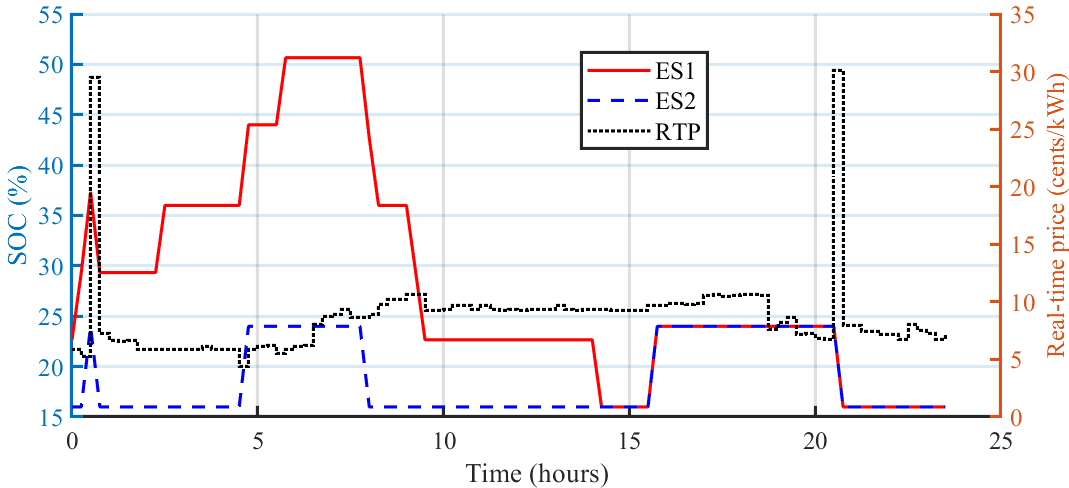
\includegraphics[width = \linewidth]{figs/A82/OFFLINE1_NM_ES.png}
\caption{Offline one day ES results with NYISO based RTP}
\label{fig:OFFLINE1_NM_ES}
\end{figure}

\begin{figure}[!ht]
\centering
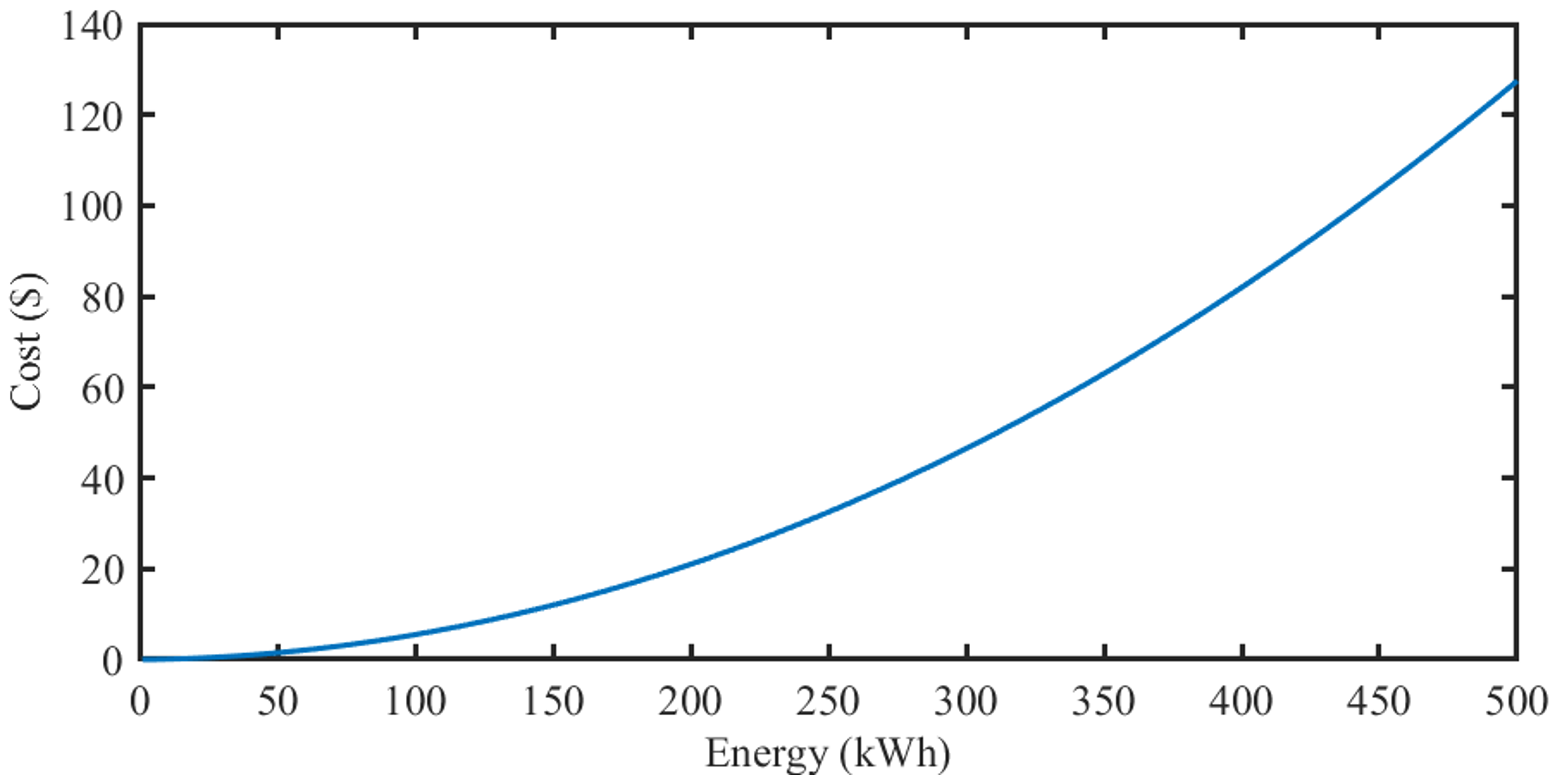
\includegraphics[width = \linewidth]{figs/A82/GEN_COST_CURVE.png}
\caption{Cost curve of the generator}
\label{fig:GEN_COST_CURVE}
\end{figure}

\begin{figure}[!ht]
\centering
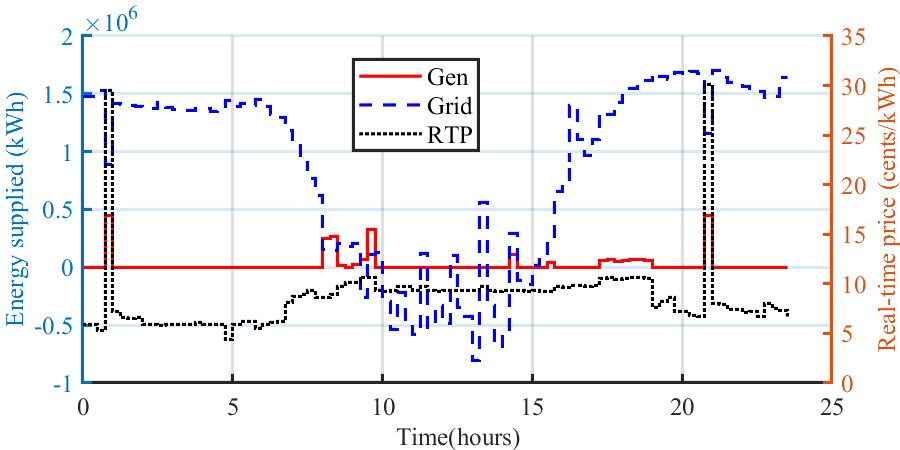
\includegraphics[width = \linewidth]{figs/A82/OFFLINE1_NM_GEN.png}
\caption{Offline one day gen and grid results with NYISO based RTP}
\label{fig:OFFLINE1_NM_Gen}
\end{figure}

\begin{figure}[!ht]
\centering
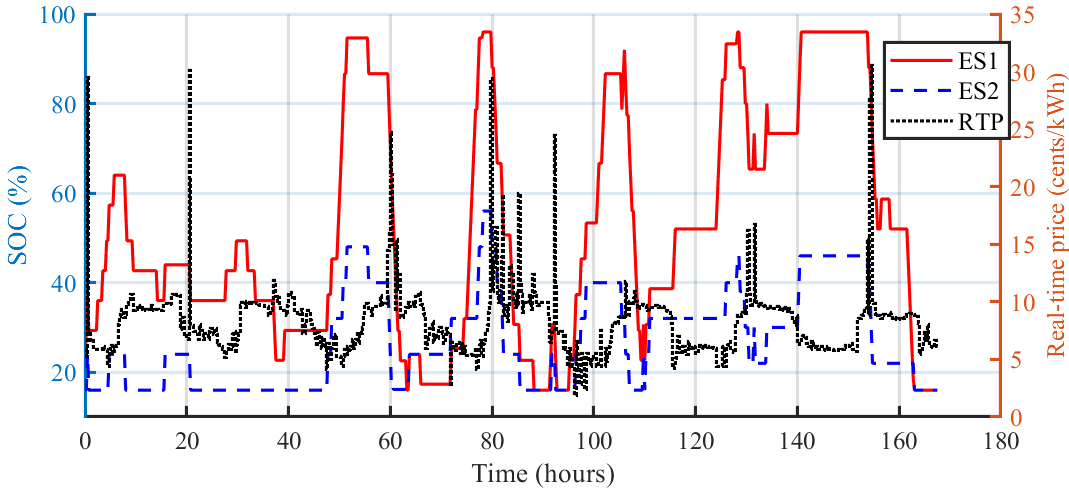
\includegraphics[width = \linewidth]{figs/A82/OFF_7_day_NYISO_ES.png}
\caption{Offline ES results with NYISO based RTP for seven days}
\label{fig:OFF_7_day_NYISO_ES}
\end{figure}


\begin{figure}[!ht]
\centering
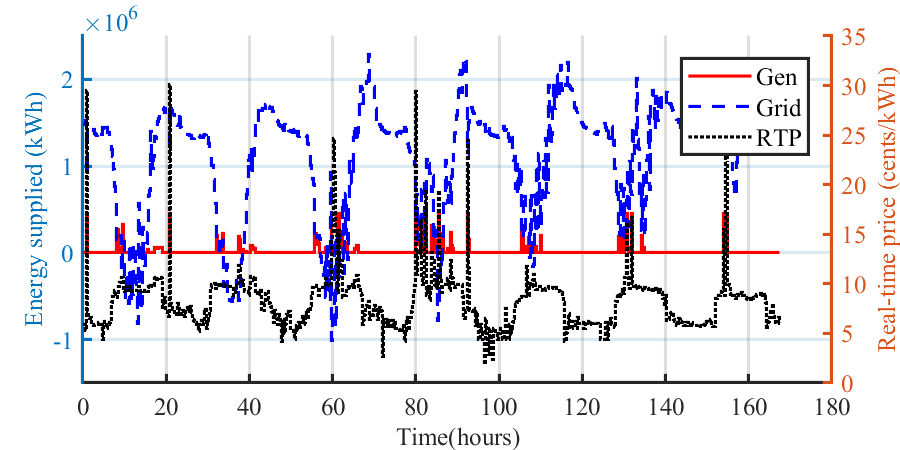
\includegraphics[width = \linewidth]{figs/A82/OFF_7_day_NYISO_GEN.png}
\caption{Offline gen and grid results with NYISO based RTP for seven days}
\label{fig:OFF_7_day_NYISO_GEN}
\end{figure}

\begin{figure}[!ht]
\centering
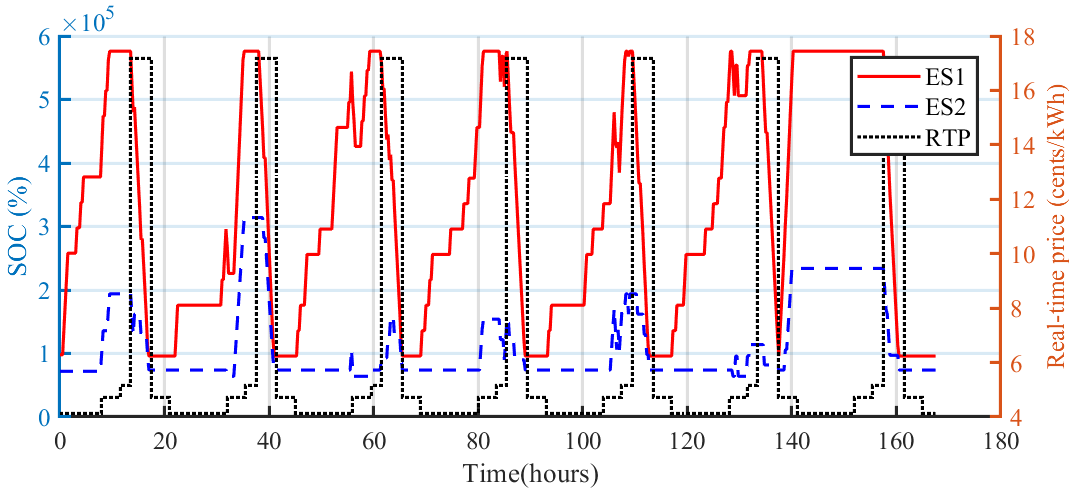
\includegraphics[width = \linewidth]{figs/A82/OFF_7_day_PGNE_ES.png}
\caption{Offline ES results with PG\&E based RTP for seven days}
\label{fig:OFF_7_day_PGNE_ES}
\end{figure}


\begin{figure}[!ht]
\centering
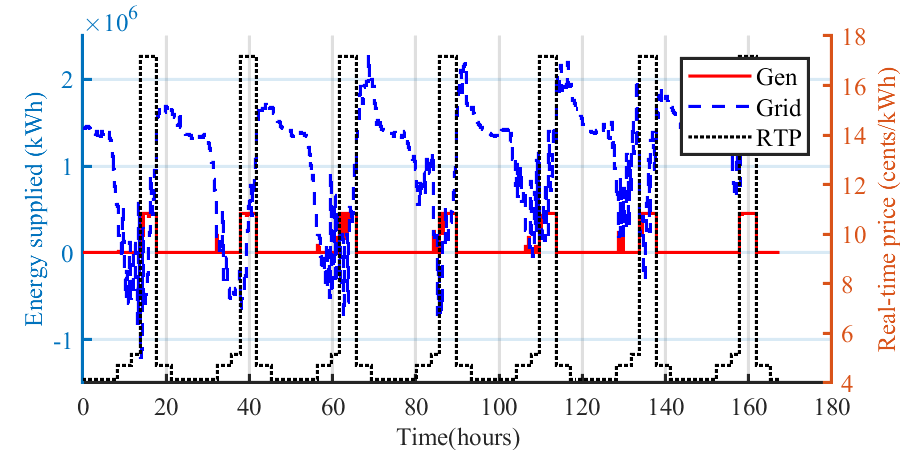
\includegraphics[width = \linewidth]{figs/A82/OFF_7_day_PGNE_GEN.png}
\caption{Offline gen and grid results with PG\&E based RTP for seven days}
\label{fig:OFF_7_day_PGNE_GEN}
\end{figure}

To validate the efficiency of the algorithm the previously mentioned NYISO and PG\&E RTP scenarios have been tested against two test cases.

Case1 is PSO based approach. The performance of the seven day test results shown in fig. \ref{fig:OFF_7_day_NYISO_ES}, fig. \ref{fig:OFF_7_day_NYISO_GEN}, fig. \ref{fig:OFF_7_day_PGNE_ES}, and fig. \ref{fig:OFF_7_day_PGNE_GEN} have been first compared against a PSO based approach. The PSO based approach used PSO to solve a modified version of (\ref{eq:multi_all_in1_sys}). The PSO problem formulation is as follows:
minimize:
\begin{multline}
\label{eq:multi_all_in1_PSO}
    ( P_{grid}*rtp + |(P_{es}(1)*r_{es}(1)| + |(P_{es}(2)*r_{es}(2)| \\ + A*P_{Gen}^2 + B*P_{Gen} )*\Delta T
\end{multline}
Subject to:

$(\delta_1 - \delta_2)/X_{12} = P_{Grid}$

$(\delta_2 - \delta_1)/X_{12}+ (\delta_2 - \delta_3/X_{23} = P_{L2}$

$(\delta_3 - \delta_2)/X_{23}+(\delta_3 - \delta_4)/X_{34}+(\delta_3 - \delta_7)/X_{37} = P_{L3}$

$(\delta_4 - \delta_3)/X_{34}+(\delta_4 - \delta_4)/X_{45}+(\delta_4 - \delta_6)/X_{46}=P_{L4} -$

$P_{PV1} - P_{es}(1) - P_{PV}(1)$

$(\delta_5 - \delta_4)/X_{45} = P_{L5}-P_{Gen}$

$(\delta_6 - \delta_4)/X_{46} = P_{L6}$

$(\delta_7 - \delta_3)/X_{37} + (\delta_7 - \delta_8)/X_{78}  = P_{L7}$

$(\delta_8 - \delta_7)/X_{78} + (\delta_8 - \delta_9)/X_{89}  = P_{L8} - P_{es}(2) - P_{PV}(2)$

$(\delta_9 - \delta_8)/X_{89} = -P_{PV}(3)$

$0 \leq P_{Gen} \leq \overline{P_{Gen}}$

$\underline{ES(1)} \leq ES_{current}(1)+(P_{es}(1)*\Delta T) \leq \overline{ES(1)}$

$\underline{ES(2)} \leq ES_{current}(2)+(P_{es}(2)*\Delta T) \leq \overline{ES(2)}$

$\underline{P_{ES}(1)} \leq P_{es}(1) \leq \overline{P_{ES}(1)}$

$\underline{P_{ES}(2)} \leq P_{es}(2) \leq \overline{P_{ES}(2)}$\\


Equation (\ref{eq:multi_all_in1_PSO}) is solved using the matlab 'particleswarm' solver \cite{MW_PSO}. The PSO based case performed much slower than the graph search based approach in this case. The comparison between all the cases are presented in table \ref{tab:Cost_MULTI}. It can be observed from the table that the PSO based approach is 4.3\% to 4.5\% less efficient compared to the graph search solution case. It can also be seen that where the graph search based solution takes an average of around 211 S to 234 s on average to finish calculation for one time-step (15  minutes), and the PSO based approach takes around 521 S to 462 s on average to finish the same calculation. In this case, it is evident that the graph search based solution provides a more cost efficient result in less time.

Case2 is GA based approach. In the GA based approach, the genetic algorithm solver available in matlab global minimum solver \cite{MW_GA} is used to solve (\ref{eq:multi_all_in1_PSO}) for each time-step. The cost and time taken for calculation for the GA case is shown in Table \ref{tab:Cost_MULTI}. It can be seen from the table that the GA based approach is 3.1\% to 3.2\% less efficient compared to the graph search solution case. The GA based case also takes around 921 S to 913 s on average to finish the calculations. This is a lot more time required to do the calculations and it is over the allotted time-step of 900s to finish the calculation. Compared to the graph search based approach the GA based approach is a lot less time efficient in this case. In fact, taking over 900 s to complete calculations for 900 s long time steps makes the approach not suitable for real-time calculation on the field.

\begin{table}
\caption{Seven day comparison between graph search, PSO, and GA based approach}
\label{tab:Cost_MULTI}
\begin{tabular}{l|l|l|}
\cline{2-3}
                                                        & NYISO                   & PG\&E                \\ \hline
\multicolumn{1}{|l|}{PSO}                               & Cost = 481,102.47185 \$ & Cost = 578,430.01 \$ \\ 
\multicolumn{1}{|l|}{}                                  & Time = 521 s            & Time = 462 s         \\ \hline
\multicolumn{1}{|l|}{GA}                                & Cost = 476,028.52 \$    & Cost =570,680.70 \$  \\ 
\multicolumn{1}{|l|}{}                                  & Time = 921 s            & Time = 913 s         \\ \hline
\multicolumn{1}{|l|}{Graph search}                      & Cost=461,267.95 \$      & Cost=553,521.54 \$   \\ 
\multicolumn{1}{|c|}{}                                  & Time = 234 s          & Time = 211 s       \\ \hline
\multicolumn{1}{|l|}{Cost saving wrt PSO (\%)} & 4.30\%                  & 4.50\%               \\ \hline
\multicolumn{1}{|l|}{Cost saving wrt GA (\%)}  & 3.20\%                  & 3.10\%               \\ \hline
\end{tabular}
\end{table}

\subsection{Effects of Discretization and Time-Step}
In the tests performed before, the ES SOCs were discretized using steps of 2\% and the time step was set to 15 minutes. This part shows the effects of changing discretization and time-steps on both time and cost. Table \ref{tab:MULTI_TIME_DELTA} shows the effect changing discretization and time-step. It shows seven day offline test results using the NYISO price profile for 2\%, 3\%, and 5\% discretization and 15 minute, 30 minute, and 60 minute time steps. The results clearly show that increasing time-step or discretization values result in less time to get a solution but it also results in a higher cost.
\begin{table}[htb]
\caption{Effects of discretization and time-step on the algorithm performance}
\centering
\label{tab:MULTI_TIME_DELTA}
\begin{tabular}{|l|l|l|l|}
\hline
Discretization & 15 minute & 30 minute & 60 minute \\ \hline
2\% ES capacity & \begin{tabular}[c]{@{}l@{}}Cost: \$461,267.95
\\ Time: 234.1
s\end{tabular} & \begin{tabular}[c]{@{}l@{}}Cost: \$480,179.93
\\ Time: 131.1s\end{tabular} & \begin{tabular}[c]{@{}l@{}}Cost: \$507,070.01
\\ Time: 49.16s\end{tabular} \\ \hline

3\% ES capacity & \begin{tabular}[c]{@{}l@{}}Cost: \$475,105.98
\\ Time: 159.18s\end{tabular} & \begin{tabular}[c]{@{}l@{}}Cost: \$494,585.33
\\ Time: 89.15s\end{tabular} & \begin{tabular}[c]{@{}l@{}}Cost: \$522,282.11
\\ Time: 33.42s\end{tabular} \\ \hline

5\% ES capacity & \begin{tabular}[c]{@{}l@{}}Cost: \$483,408.81
\\ Time: 56.18s\end{tabular} & \begin{tabular}[c]{@{}l@{}}Cost: \$503,228.57
\\ Time: 31.46s\end{tabular} & \begin{tabular}[c]{@{}l@{}}Cost: \$531,409.373
\\ Time: 11.79s\end{tabular} \\ \hline
\end{tabular}
\end{table}

\subsection{Starting With Different SOC}
Similar to the previous chapter the ES1 and ES2 are started from a SOC of 50\% and 24\%. The responses of ES1 and ES2 are shown in  fig. \ref{fig:OFF_DIFF_SOC_ES12}. It can be seen that similar to the single ES example shown in the previous chapter, ES1 ans ES2 are taking into account the extra starting energy to decide the charging and discharging actions. Fig. \ref{fig:OFF_DIFF_SOC_GRID_GEN} shows the response of the generator and grid. It can be seen that the generator response does not depend on the starting position of the ES. It has the same response as fig. \ref{fig:OFFLINE1_NM_Gen}.

\begin{figure}[!ht]
\centering
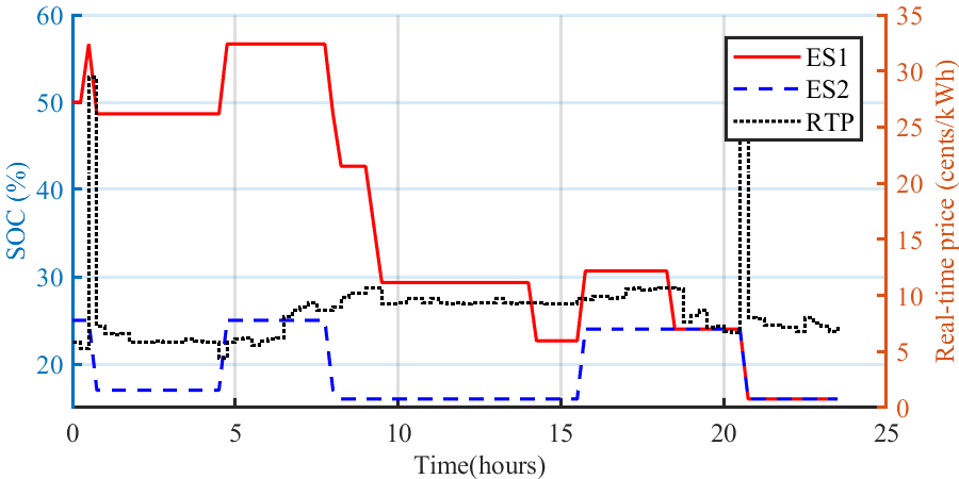
\includegraphics[width = \linewidth]{figs/A82/OFF_DIFF_SOC_ES12.png}
\caption{Starting from different SOC, ES1 and ES2 responses.}
\label{fig:OFF_DIFF_SOC_ES12}
\end{figure}

\begin{figure}[!ht]
\centering
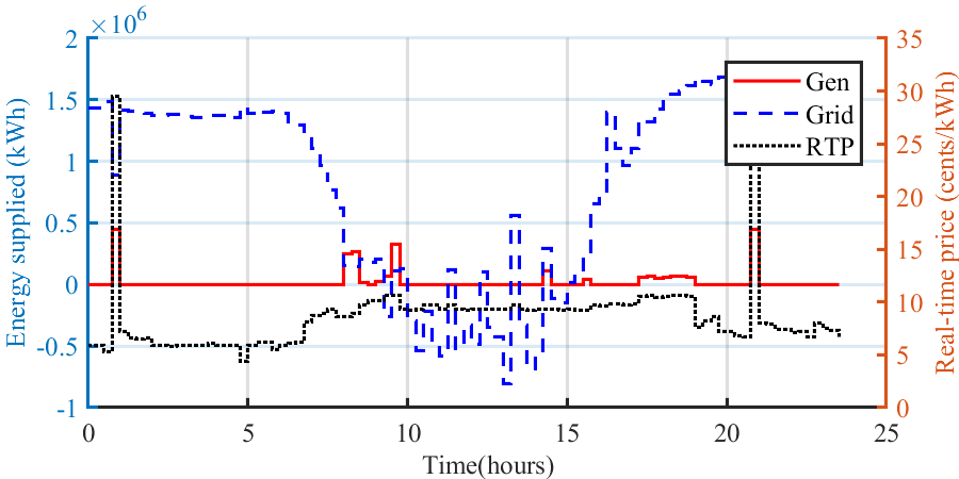
\includegraphics[width = \linewidth]{figs/A82/OFF_DIFF_SOC_GRID_GEN.png}
\caption{Starting from different SOC, generator and grid responses.}
\label{fig:OFF_DIFF_SOC_GRID_GEN}
\end{figure}


\section{Real-Time Validation and Results}
The process used for real-time validation is the same as chapter \ref{A8_cahp}. The CHIL testbed and controller hardware setup was the same. The model used in the DRTS was modeled using the same methodologies. The real-time validation also uses the same DNP3 communication over TCP/IP. For the first CHIL validation, the one day simulation scenario using the NYISO RTP described in the previous section was used. Fig. \ref{fig:OFFLINE1_NM_ES1_Z_RT} shows the real-time vs offline responses comparison for ES1. The blue solid line is the offline response and the dotted black line is the real-time response. The responses differ 0.3\% which is negligible. Fig. \ref{fig:OFFLINE1_NM_ES2_Z_RT}, and fig. \ref{fig:OFFLINE1_NM_GEN_Z_RT} shows the offline vs real-time responses for ES2 and the generator. In both cases, the dotted black line is the real-time response and the solid blue line is the offline response. They show a difference of 0.13\% and 0.014\% respectively. This is expected as similar to Chapter \ref{A8_cahp} offline simulation models were modeled for phasor simulation and the real-time simulation models were modeled for electromagnetic transient program simulation.

\begin{figure}[!ht]
\centering
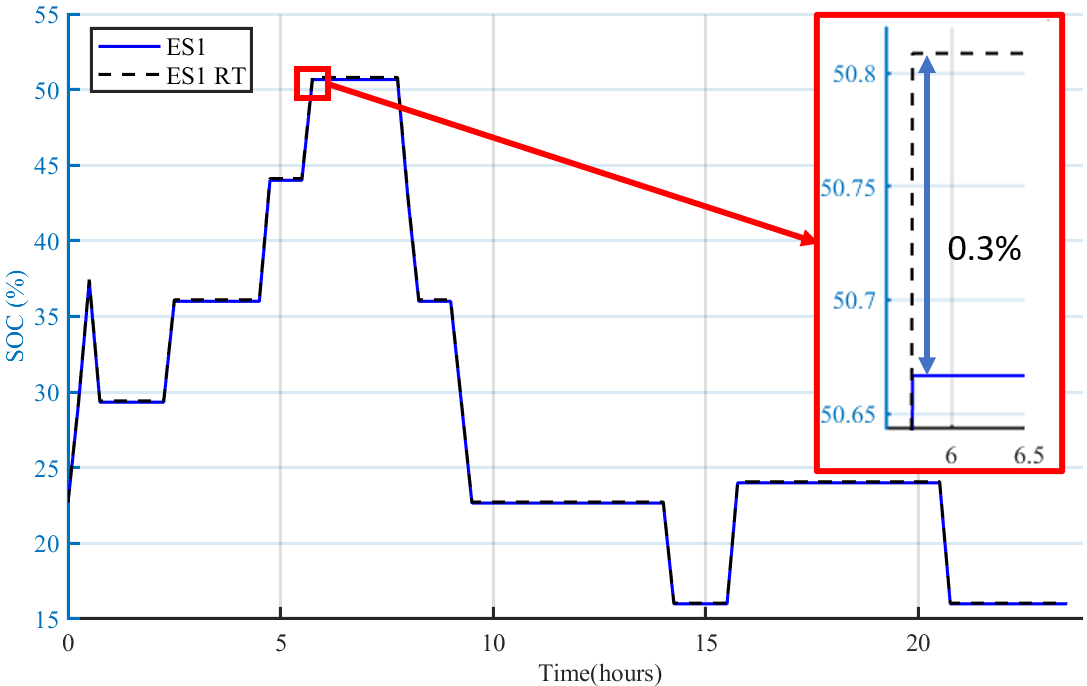
\includegraphics[width = \linewidth]{figs/A82/OFFLINE1_NM_ES1_Z_RT.png}
\caption{Comparison between ES1 responses, real-time vs offline (NYISO).}
\label{fig:OFFLINE1_NM_ES1_Z_RT}
\end{figure}

\begin{figure}[!ht]
\centering
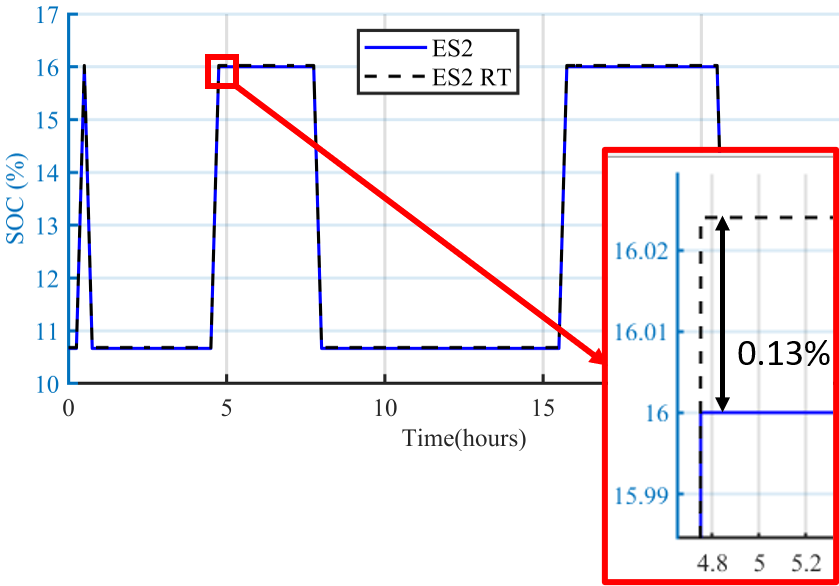
\includegraphics[width = \linewidth]{figs/A82/OFFLINE1_NM_ES2_Z_RT.png}
\caption{Comparison between ES2 responses, real-time vs offline (NYISO).}
\label{fig:OFFLINE1_NM_ES2_Z_RT}
\end{figure}

\begin{figure}[!ht]
\centering
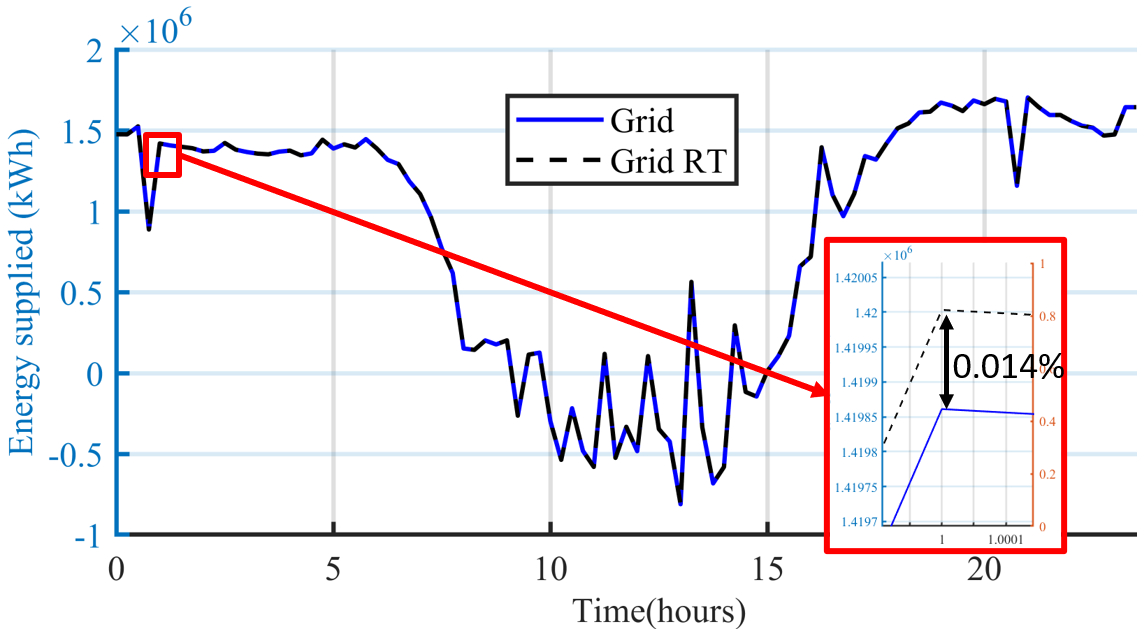
\includegraphics[width = \linewidth]{figs/A82/OFFLINE1_NM_GEN_Z_RT.png}
\caption{Comparison between generator responses, real-time vs offline (NYISO).}
\label{fig:OFFLINE1_NM_GEN_Z_RT}
\end{figure}

The second CHIL validation uses the PG\&E based RTP. Fig. \ref{fig:PGNE1_NM_ES1_Z_RT}, Fig. \ref{fig:PGNE1_NM_ES2_Z_RT}, and Fig. \ref{fig:PGNE1_NM_GEN_Z_RT} shows the offline and real-time response for ES1, ES2, and the generator, respectively. The dotted black line represents the real-time response and the solid blue line represents the off-line response in all the figures. The offline vs real-time difference for ES1, ES2, and generator are 0.2\%, 0.25\%, and 0.017\% respectively. These differences are negligible. This verifies the algorithm's capabilities to operate in a real-time environment.

\begin{figure}[!ht]
\centering
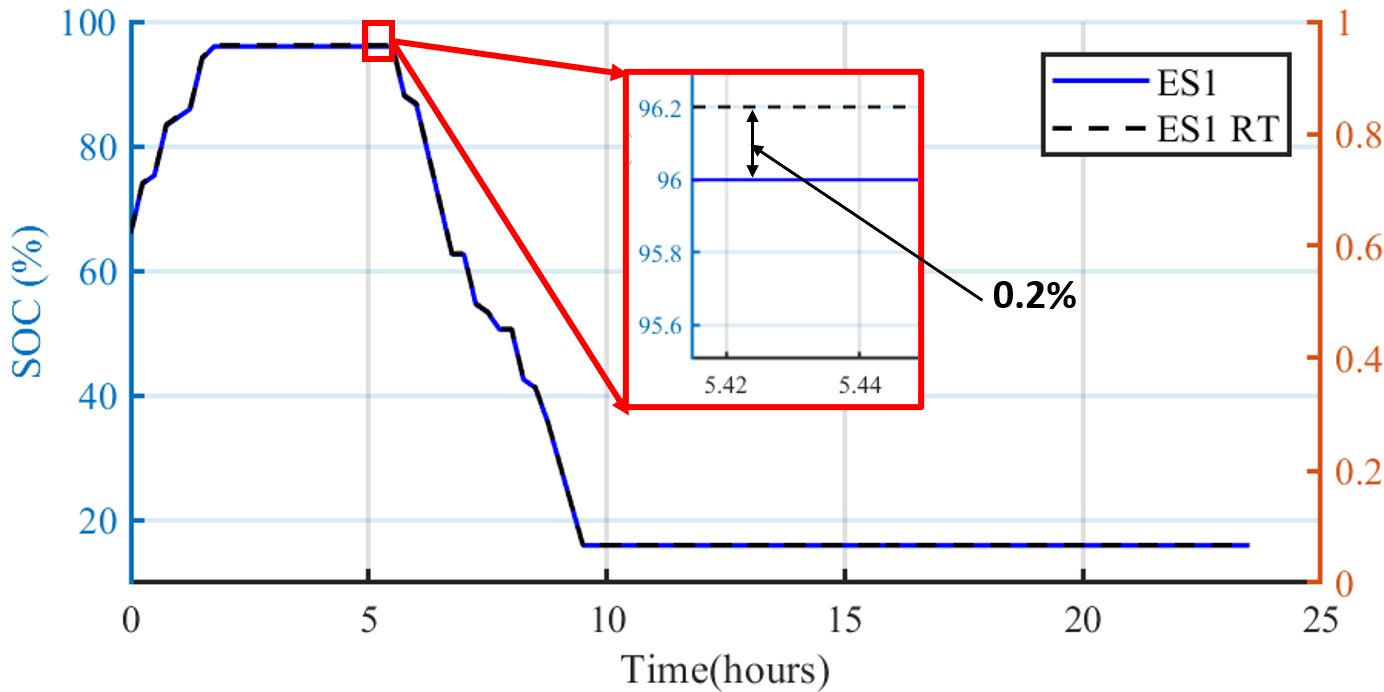
\includegraphics[width = \linewidth]{figs/A82/PGNE_RT_OFF_ES1.png}
\caption{Comparison between ES1 responses, real-time vs offline (PG\&E).}
\label{fig:PGNE1_NM_ES1_Z_RT}
\end{figure}

\begin{figure}[!ht]
\centering
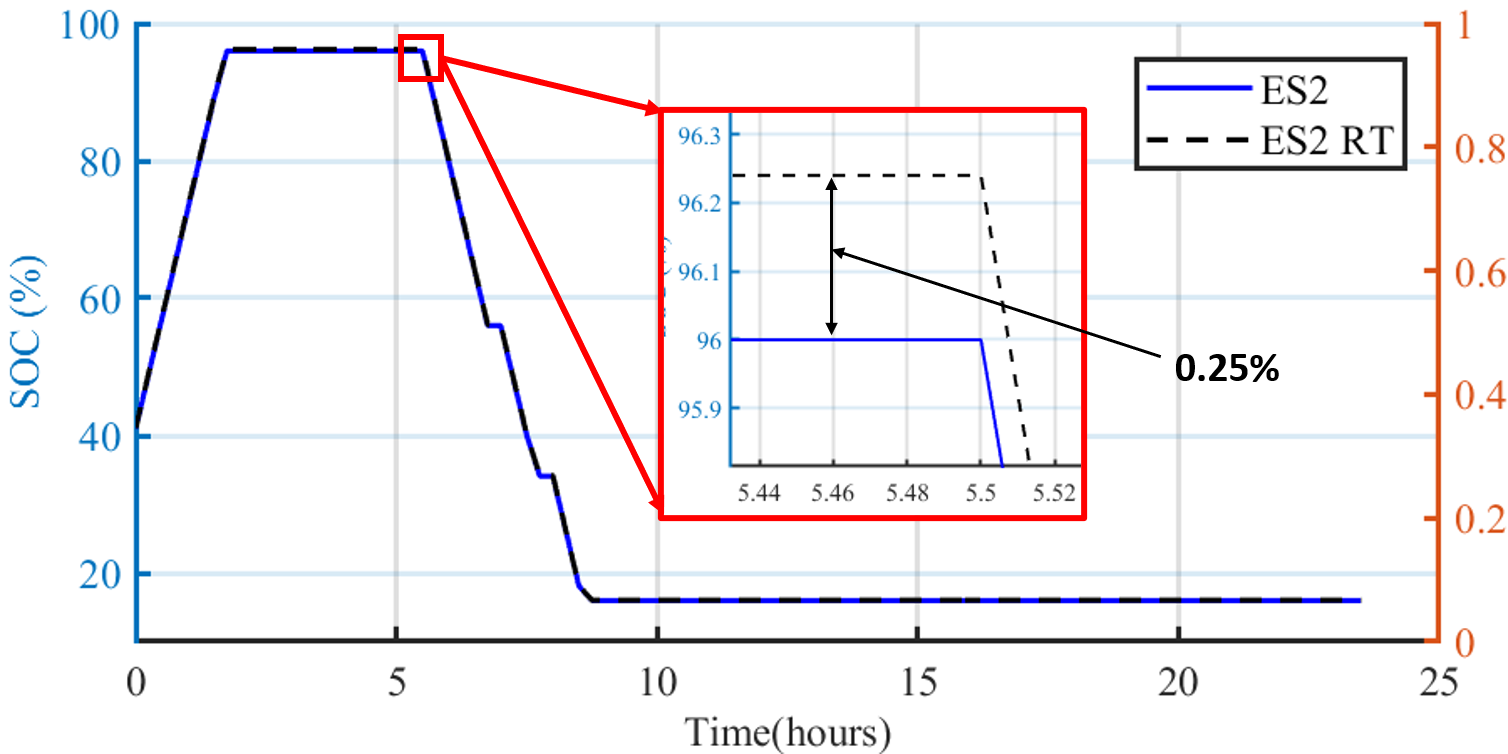
\includegraphics[width = \linewidth]{figs/A82/PGNE_RT_OFF_ES2.png}
\caption{Comparison between ES2 responses, real-time vs offline (PG\&E).}
\label{fig:PGNE1_NM_ES2_Z_RT}
\end{figure}

\begin{figure}[!ht]
\centering
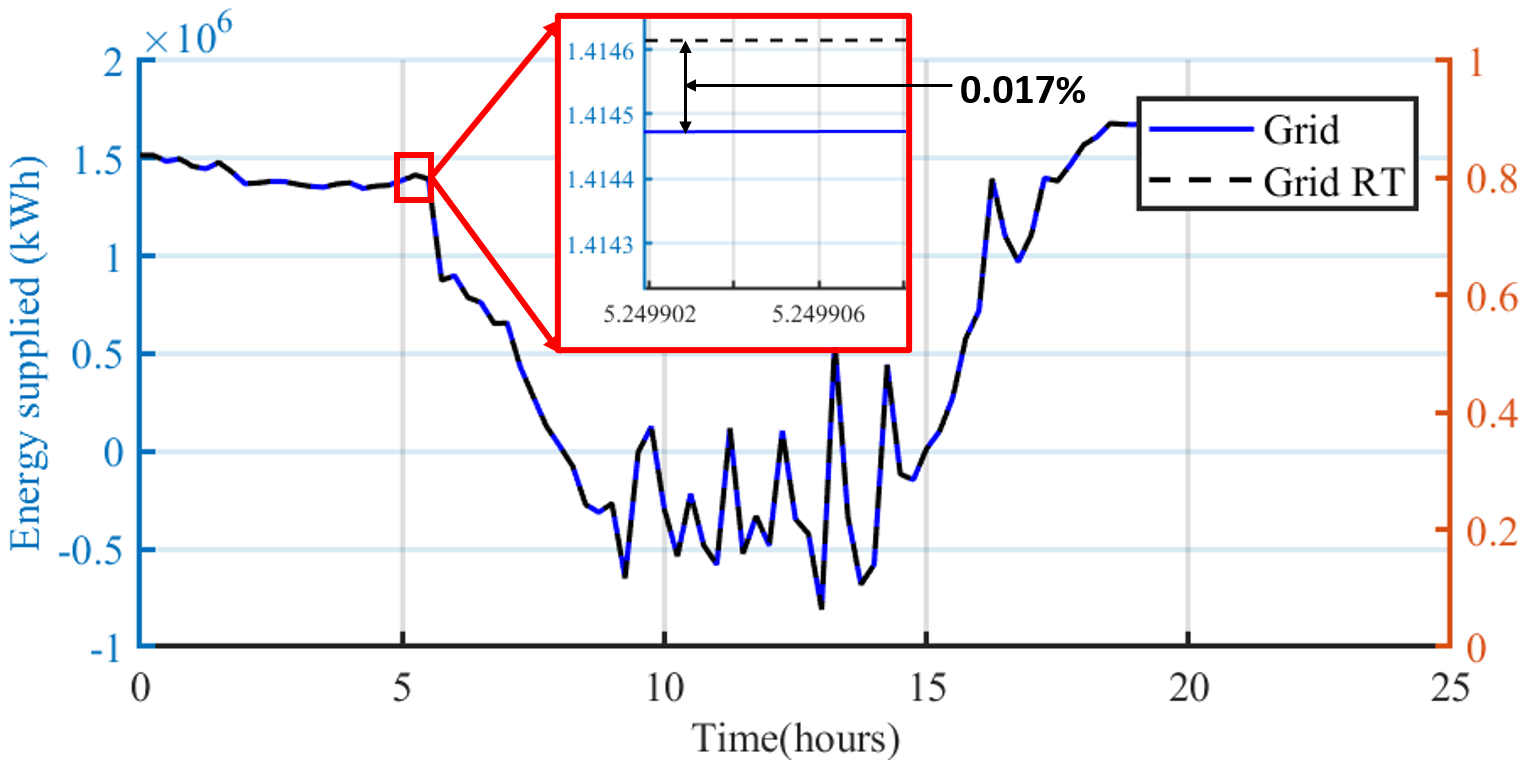
\includegraphics[width = \linewidth]{figs/A82/PGNE_RT_OFF_GEN.png}
\caption{Comparison between generator responses, real-time vs offline (PG\&E).}
\label{fig:PGNE1_NM_GEN_Z_RT}
\end{figure}

\section{Conclusion}
In this chapter, an energy management solution for DERs contained in a distribution grid or a microgrid is discussed. The solution is based on the graph search based solution discussed in Chapter \ref{A8_cahp} and uses DC power-flow and quadratic programming to get the most cost optimum solution. The algorithm has been verified against GA and PSO based methods offline. The proposed algorithm shows significant gains in terms of time needed to complete calculations and cost savings. It is also shown that the algorithm can be modified to get faster calculation time sacrificing cost savings. This trait makes the algorithm tune able based on the specifications of the problem. Finally, the algorithm was validated using CHIL and the validation shows negligible difference from the offline behaviour.


\bibliographystyle{IEEEtran}
\bibliography{mybib.bib}

% \ifCLASSOPTIONcaptionsoff
%   \newpage
% \fi

\end{document}
